% Options for packages loaded elsewhere
\PassOptionsToPackage{unicode}{hyperref}
\PassOptionsToPackage{hyphens}{url}
%
\documentclass[
  ignorenonframetext,
]{beamer}
\usepackage{pgfpages}
\setbeamertemplate{caption}[numbered]
\setbeamertemplate{caption label separator}{: }
\setbeamercolor{caption name}{fg=normal text.fg}
\beamertemplatenavigationsymbolsempty
% Prevent slide breaks in the middle of a paragraph
\widowpenalties 1 10000
\raggedbottom
\setbeamertemplate{part page}{
  \centering
  \begin{beamercolorbox}[sep=16pt,center]{part title}
    \usebeamerfont{part title}\insertpart\par
  \end{beamercolorbox}
}
\setbeamertemplate{section page}{
  \centering
  \begin{beamercolorbox}[sep=12pt,center]{part title}
    \usebeamerfont{section title}\insertsection\par
  \end{beamercolorbox}
}
\setbeamertemplate{subsection page}{
  \centering
  \begin{beamercolorbox}[sep=8pt,center]{part title}
    \usebeamerfont{subsection title}\insertsubsection\par
  \end{beamercolorbox}
}
\AtBeginPart{
  \frame{\partpage}
}
\AtBeginSection{
  \ifbibliography
  \else
    \frame{\sectionpage}
  \fi
}
\AtBeginSubsection{
  \frame{\subsectionpage}
}

\usepackage{amsmath,amssymb}
\usepackage{iftex}
\ifPDFTeX
  \usepackage[T1]{fontenc}
  \usepackage[utf8]{inputenc}
  \usepackage{textcomp} % provide euro and other symbols
\else % if luatex or xetex
  \usepackage{unicode-math}
  \defaultfontfeatures{Scale=MatchLowercase}
  \defaultfontfeatures[\rmfamily]{Ligatures=TeX,Scale=1}
\fi
\usepackage{lmodern}
\ifPDFTeX\else  
    % xetex/luatex font selection
\fi
% Use upquote if available, for straight quotes in verbatim environments
\IfFileExists{upquote.sty}{\usepackage{upquote}}{}
\IfFileExists{microtype.sty}{% use microtype if available
  \usepackage[]{microtype}
  \UseMicrotypeSet[protrusion]{basicmath} % disable protrusion for tt fonts
}{}
\makeatletter
\@ifundefined{KOMAClassName}{% if non-KOMA class
  \IfFileExists{parskip.sty}{%
    \usepackage{parskip}
  }{% else
    \setlength{\parindent}{0pt}
    \setlength{\parskip}{6pt plus 2pt minus 1pt}}
}{% if KOMA class
  \KOMAoptions{parskip=half}}
\makeatother
\usepackage{xcolor}
\newif\ifbibliography
\setlength{\emergencystretch}{3em} % prevent overfull lines
\setcounter{secnumdepth}{-\maxdimen} % remove section numbering


\providecommand{\tightlist}{%
  \setlength{\itemsep}{0pt}\setlength{\parskip}{0pt}}\usepackage{longtable,booktabs,array}
\usepackage{calc} % for calculating minipage widths
\usepackage{caption}
% Make caption package work with longtable
\makeatletter
\def\fnum@table{\tablename~\thetable}
\makeatother
\usepackage{graphicx}
\makeatletter
\def\maxwidth{\ifdim\Gin@nat@width>\linewidth\linewidth\else\Gin@nat@width\fi}
\def\maxheight{\ifdim\Gin@nat@height>\textheight\textheight\else\Gin@nat@height\fi}
\makeatother
% Scale images if necessary, so that they will not overflow the page
% margins by default, and it is still possible to overwrite the defaults
% using explicit options in \includegraphics[width, height, ...]{}
\setkeys{Gin}{width=\maxwidth,height=\maxheight,keepaspectratio}
% Set default figure placement to htbp
\makeatletter
\def\fps@figure{htbp}
\makeatother

\makeatletter
\@ifpackageloaded{caption}{}{\usepackage{caption}}
\AtBeginDocument{%
\ifdefined\contentsname
  \renewcommand*\contentsname{Table of contents}
\else
  \newcommand\contentsname{Table of contents}
\fi
\ifdefined\listfigurename
  \renewcommand*\listfigurename{List of Figures}
\else
  \newcommand\listfigurename{List of Figures}
\fi
\ifdefined\listtablename
  \renewcommand*\listtablename{List of Tables}
\else
  \newcommand\listtablename{List of Tables}
\fi
\ifdefined\figurename
  \renewcommand*\figurename{Figure}
\else
  \newcommand\figurename{Figure}
\fi
\ifdefined\tablename
  \renewcommand*\tablename{Table}
\else
  \newcommand\tablename{Table}
\fi
}
\@ifpackageloaded{float}{}{\usepackage{float}}
\floatstyle{ruled}
\@ifundefined{c@chapter}{\newfloat{codelisting}{h}{lop}}{\newfloat{codelisting}{h}{lop}[chapter]}
\floatname{codelisting}{Listing}
\newcommand*\listoflistings{\listof{codelisting}{List of Listings}}
\makeatother
\makeatletter
\makeatother
\makeatletter
\@ifpackageloaded{caption}{}{\usepackage{caption}}
\@ifpackageloaded{subcaption}{}{\usepackage{subcaption}}
\makeatother
\ifLuaTeX
  \usepackage{selnolig}  % disable illegal ligatures
\fi
\usepackage{bookmark}

\IfFileExists{xurl.sty}{\usepackage{xurl}}{} % add URL line breaks if available
\urlstyle{same} % disable monospaced font for URLs
\hypersetup{
  pdftitle={Basis and Linear Independence},
  pdfauthor={Jeremy Teitelbaum},
  hidelinks,
  pdfcreator={LaTeX via pandoc}}

\title{Basis and Linear Independence}
\author{Jeremy Teitelbaum}
\date{}

\begin{document}
\frame{\titlepage}

\begin{frame}{Basis}
\phantomsection\label{basis}
A set of vectors in \(\mathbf{R}^{n}\) (or in any vector space \(V\)) is
called a \textbf{basis} if

\begin{itemize}
\tightlist
\item
  it spans \(V\)
\item
  it is linearly independent.
\end{itemize}

Examples: if \(A\) is an invertible \(n\times n\) matrix, its columns
are linearly independent and span \(\mathbf{R}^{n}\) and therefore are a
basis for \(\mathbf{R}^{n}\).

The vectors \(1,x,x^2,\ldots, x^n\) span the polynomials of degree at
most \(n\) and are linearly indepenent.

The ``standard vectors'' \(e_{i}\) for \(i=1,\ldots, n\) are a basis for
\(\mathbf{R}^{n}\).
\end{frame}

\begin{frame}{Subspace basis}
\phantomsection\label{subspace-basis}
The vectors \((1,3,2)\) and \((-1,-1,0)\) are linearly indepedent and
span a subspace \(H\) of \(\mathbf{R}^{3}\).

Therefore they are a basis for \(H\).
\end{frame}

\begin{frame}{Every spanning set contains a basis}
\phantomsection\label{every-spanning-set-contains-a-basis}
If a set \(S\) of vectors \(v_1,\ldots, v_n\) spans a subspace \(H\),
then a subset of \(S\) is a basis.

\textbf{Proof:} If the vectors are linearly indepenent, they are already
a basis.

If they are dependent, then one is a linear combination of the others.
Remove that one from \(S\). The result still spans.

Continue removing dependent vectors until the remaining vectors are
independent, and you've found your basis.
\end{frame}

\begin{frame}{A basis is a minimal spanning set}
\phantomsection\label{a-basis-is-a-minimal-spanning-set}
If \(H\) is a subspace of \(V\), suppose you have a bunch of vectors in
\(H\).

Too many vectors makes them dependent. To few means they can't span. If
they are a basis, there are enough to span, but not to become dependent.
\end{frame}

\begin{frame}{Basis for \(\mathrm{Nul}(A)\).}
\phantomsection\label{basis-for-mathrmnula.}
The null space of \(A\) is spanned by the vectors with weights given by
the free variables in the row reduced from of \(A\).

Those vectors are independent and therefore form a basis.
\end{frame}

\begin{frame}{Basis for \(\mathrm{Col}(A)\).}
\phantomsection\label{basis-for-mathrmcola.}
Given vectors \(v_1,\ldots, v_k\), make an \(m\times k\) matrix with the
\(v_{i}\) as columns.

To find a linear relation among the columns of \(A\), we need to solve
\(Ax=0\).

But \(Ax=0\) if and only if \(EAx=0\) where \(E\) is an elementary
matrix.

Put another way, row reduction doesn't change the \(x\) such that
\(Ax=0\).

So we can assume \(A\) is in row reduced echelon form.
\end{frame}

\begin{frame}{More on basis for \(\mathrm{Col}(A)\).}
\phantomsection\label{more-on-basis-for-mathrmcola.}
Once \(A\) is in row reduced form, we see that:

\begin{itemize}
\item
  the columns corresponding to free variables are linear combinations of
  the pivot columns
\item
  the pivot columns are linearly independent.
\end{itemize}
\end{frame}

\begin{frame}{Basis for \(\mathrm{Col}(A)\).}
\phantomsection\label{basis-for-mathrmcola.-1}
The \textbf{columns of \(A\)} corresponding to the pivot columns in the
row reduced version of \(A\) are a basis for the column space. (note
that these are \emph{not} the columns of the reduced matrix).

So: a basis for the null space is made up of \(k\) vectors where \(k\)
is the number of free variables, and a basis for the column space is
made up of \(r\) vectors where \(r\) is the number of pivot columns.

Notice that \(k+r=n\) where \(n\) is the total number of columns of
\(A\).
\end{frame}

\begin{frame}{Example}
\phantomsection\label{example}
Suppose that

\[
A=\left[\begin{matrix} 2 & 4 & 5& 1\\ 1 & -3 & -2& 0\\ 0 & -2 & -3 & 1\end{matrix}\right]
\]

The row reduced form of \(A\) is \[
\left[\begin{matrix}1 & 0 & 0 & 1 \\ 0 & 1 & 0 & 1\\0 & 0 & 1 & -1\end{matrix}\right]
\]

Since the first three columns are pivot columns, the first three columns
of \(A\) span the column space of \(A\), and the last column satisfies
\(c_4 = c_1+c_2-c_3\).
\end{frame}

\begin{frame}{Example continued}
\phantomsection\label{example-continued}
The nullspace of \(A\) is the solution to the homogeneous system, and it
is given by the equations \[\begin{array}{ccc}
x_1 &=&-x_4 \\
x_2 &=& -x_4 \\
x_3 &=& x_4
\end{array}
\]

so the null space is spanned by \[
\left[\begin{matrix} -1 \\ -1 \\ 1 \\ 1\end{matrix}\right]
\]
\end{frame}

\begin{frame}{Null Space and Col Space}
\phantomsection\label{null-space-and-col-space}
\begin{figure}[H]

{\centering 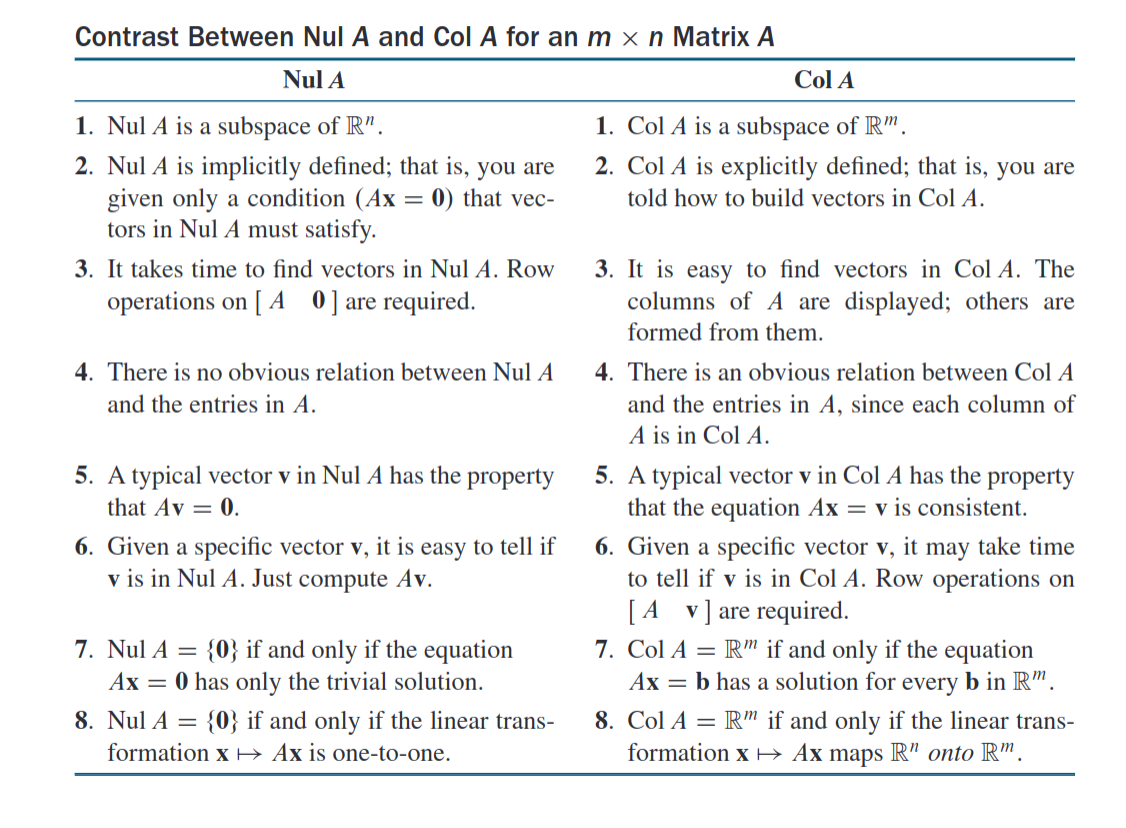
\includegraphics{NulvsCol.png}

}

\caption{Null Space vs Col Space}

\end{figure}%
\end{frame}

\begin{frame}{Row space}
\phantomsection\label{row-space}
The \emph{row space} of a matrix is the span of its rows.

Row operations do not change the row space, so one can find a basis for
the row space of \(A\) by putting \(A\) in reduced form.

The rows with a pivot (that is, the nonzero rows) form a basis for the
row space.

This is because they are clearly linearly independent (and they span by
definition).
\end{frame}

\begin{frame}{Linear Transformations}
\phantomsection\label{linear-transformations}
A linear transformation (or linear map) \(T:V\to W\), where \(V\) and
\(W\) are vector spaces, is a function that satisfies
\(T(u+v)=T(u)+T(v)\) and \(T(cv)=cT(v)\) for all \(u,v\in V\) and
\(c\in\mathbf{R}\).

The \emph{kernel} of a linear transformation is the set of vectors that
map to zero: \[
\mathrm{kernel}(T)=\{x\in V: T(x)=0\bar}\]

The \emph{range} or \emph{image} of a linear transformation is the set
of vectors \(w\in W\) such that there is a \(v\in V\) with \(T(v)=w\).
\end{frame}

\begin{frame}{Coordinate systems}
\phantomsection\label{coordinate-systems}
\textbf{Unique representation:} Suppose that \(B=\{b_1,\ldots, b_n\}\)
are a basis for a vector space \(V\). Then any vector \(v\) can be
written in exactly one way as a linear combination of the \(b_{i}\): \[
v = c_1 b_1+\ldots+c_n b_n
\]

The coefficients \(c_1,\ldots, c_n\) are called the \emph{coordinates}
of \(v\) relative to the basis \(B\).

The vector \[
\left[\begin{matrix} c_1 \\ \vdots \\ c_n\end{matrix}\right]
\] is called the \emph{coordinate vector} for \(v\) relative to \(B\).
\end{frame}



\end{document}
